%  template.tex for Biometrics papers
%
%  This file provides a template for Biometrics authors.  Use this
%  template as the starting point for creating your manuscript document.
%  See the file biomsample.tex for an example of a full-blown manuscript.

%  ALWAYS USE THE referee OPTION WITH PAPERS SUBMITTED TO BIOMETRICS!!!
%  You can see what your paper would look like typeset by removing
%  the referee option.  Because the typeset version will be in two
%  columns, however, some of your equations may be too long. DO NOT
%  use the \longequation option discussed in the user guide!!!  This option
%  is reserved ONLY for equations that are impossible to split across
%  multiple lines; e.g., a very wide matrix.  Instead, type your equations
%  so that they stay in one column and are split across several lines,
%  as are almost all equations in the journal.  Use a recent version of the
%  journal as a guide.
%
\documentclass[useAMS,usenatbib,referee]{biom}
%documentclass[useAMS]{biom}
%
%  If your system does not have the AMS fonts version 2.0 installed, then
%  remove the useAMS option.
%
%  useAMS allows you to obtain upright Greek characters.
%  e.g. \umu, \upi etc.  See the section on "Upright Greek characters" in
%  this guide for further information.
%
%  If you are using AMS 2.0 fonts, bold math letters/symbols are available
%  at a larger range of sizes for NFSS release 1 and 2 (using \boldmath or
%  preferably \bmath).
%
%  Other options are described in the user guide. Here are a few:
%
%  -  If you use Patrick Daly's natbib  to cross-reference your
%     bibliography entries, use the usenatbib option
%
%  -  If you use \includegraphics (graphicx package) for importing graphics
%     into your figures, use the usegraphicx option
%
%  If you wish to typeset the paper in Times font (if you do not have the
%  PostScript Type 1 Computer Modern fonts you will need to do this to get
%  smoother fonts in a PDF file) then uncomment the next line
%  \usepackage{Times}

%%%%% PLACE YOUR OWN MACROS HERE %%%%%

\def\bSig\mathbf{\Sigma}
\newcommand{\VS}{V\&S}
\newcommand{\tr}{\mbox{tr}}
\newcommand{\RNum}[1]{\uppercase\expandafter{\romannumeral #1\relax}}

%packages

\usepackage{amsmath}
%\usepackage{biblatex}
\usepackage{bm}
\usepackage{hyperref}
\usepackage{graphicx}
%\usepackage{natbib}
%\usepackage{subcaption}

%  The rotating package allows you to have tables displayed in landscape
%  mode.  The rotating package is NOT included in this distribution, but
%  can be obtained from the CTAN archive.  USE OF LANDSCAPE TABLES IS
%  STRONGLY DISCOURAGED -- create landscape tables only as a last resort if
%  you see no other way to display the information.  If you do do this,
%  then you need the following command.

%\usepackage[figuresright]{rotating}

%%%%%%%%%%%%%%%%%%%%%%%%%%%%%%%%%%%%%%%%%%%%%%%%%%%%%%%%%%%%%%%%%%%%%

%  Here, place your title and author information.  Note that in
%  use of the \author command, you create your own footnotes.  Follow
%  the examples below in creating your author and affiliation information.
%  Also consult a recent issue of the journal for examples of formatting.

\title[Addressing Confounding and Measurement Error]{Addressing Confounding and Exposure Measurement Error Using Conditional Score Functions}

%  Here are examples of different configurations of author/affiliation
%  displays.  According to the Biometrics style, in some instances,
%  the convention is to have superscript *, **, etc footnotes to indicate
%  which of multiple email addresses belong to which author.  In this case,
%  use the \email{ } command to produce the emails in the display.

%  In other cases, such as a single author or two authors from
%  different institutions, there should be no footnoting.  Here, use
%  the \emailx{ } command instead.

%  The examples below correspond to almost every possible configuration
%  of authors and may be used as a guide.  For other configurations, consult
%  a recent issue of the the journal.

%  Single author -- USE \emailx{ } here so that no asterisk footnoting
%  for the email address will be produced.

%\author{John Author\emailx{email@address.edu} \\
%Department of Statistics, University of Warwick, Coventry CV4 7AL, U.K.}

%  Two authors from the same institution, with both emails -- use
%  \email{ } here to produce the asterisk footnoting for each email address

%\author{John Author$^{*}$\email{author@address.edu} and
%Kathy Authoress$^{**}$\email{email2@address.edu} \\
%Department of Statistics, University of Warwick, Coventry CV4 7AL, U.K.}

%  Exactly two authors from different institutions, with both emails
%  USE \emailx{ } here so that no asterisk footnoting for the email address
%  is produced.

%\author
%{John Author\emailx{author@address.edu} \\
%Department of Statistics, University of Warwick, Coventry CV4 7AL, U.K.
%\and
%Kathy Author\emailx{anotherauthor@address.edu} \\
%Department of Biostatistics, University of North Carolina at Chapel Hill,
%Chapel Hill, North Carolina, U.S.A.}

%  Three or more authors from same institution with all emails displayed
%  and footnoted using asterisks -- use \email{ }

%\author{John Author$^*$\email{author@address.edu},
%Jane Author$^{**}$\email{jane@address.edu}, and
%Dick Author$^{***}$\email{dick@address.edu} \\
%Department of Statistics, University of Warwick, Coventry CV4 7AL, U.K}

%  Three or more authors from same institution with one corresponding email
%  displayed

%\author{John Author$^*$\email{author@address.edu},
%Jane Author, and Dick Author \\
%Department of Statistics, University of Warwick, Coventry CV4 7AL, U.K}

%  Three or more authors, with at least two different institutions,
%  more than one email displayed

%\author{John Author$^{1,*}$\email{author@address.edu},
%Kathy Author$^{2,**}$\email{anotherauthor@address.edu}, and
%Wilma Flinstone$^{3,***}$\email{wilma@bedrock.edu} \\
%$^{1}$Department of Statistics, University of Warwick, Coventry CV4 7AL, U.K \\
%$^{2}$Department of Biostatistics, University of North Carolina at
%Chapel Hill, Chapel Hill, North Carolina, U.S.A. \\
%$^{3}$Department of Geology, University of Bedrock, Bedrock, Kansas, U.S.A.}

%  Three or more authors with at least two different institutions and only
%  one email displayed

\author{Bryan S. Blette$^{1}$, Peter B. Gilbert$^{2}$, and Michael G. Hudgens$^{1,*}$\email{mhudgens@email.unc.edu} \\ $^{1}$Department of Biostatistics, University of North Carolina at Chapel Hill
\\ Chapel Hill, NC, U.S.A. \\
$^{2}$Department of Biostatistics, University of Washington and Fred Hutchinson Cancer Research Center
\\ Seattle, Washington, U.S.A.}


\usepackage{Sweave}
\begin{document}
\Sconcordance{concordance:Biometrics-draft.tex:Biometrics-draft.rnw:%
1 152 1 1 0 361 1}


%  This will produce the submission and review information that appears
%  right after the reference section.  Of course, it will be unknown when
%  you submit your paper, so you can either leave this out or put in
%  sample dates (these will have no effect on the fate of your paper in the
%  review process!)

%\date{{\it Received October} 2007. {\it Revised February} 2008.  {\it
%Accepted March} 2008.}

%  These options will count the number of pages and provide volume
%  and date information in the upper left hand corner of the top of the
%  first page as in published papers.  The \pagerange command will only
%  work if you place the command \label{firstpage} near the beginning
%  of the document and \label{lastpage} at the end of the document, as we
%  have done in this template.

%  Again, putting a volume number and date is for your own amusement and
%  has no bearing on what actually happens to your paper!

%\pagerange{\pageref{firstpage}--\pageref{lastpage}}
%\volume{64}
%\pubyear{2008}
%\artmonth{December}

%  The \doi command is where the DOI for your paper would be placed should it
%  be published.  Again, if you make one up and stick it here, it means
%  nothing!

%\doi{10.1111/j.1541-0420.2005.00454.x}

%  This label and the label ``lastpage'' are used by the \pagerange
%  command above to give the page range for the article.  You may have
%  to process the document twice to get this to match up with what you
%  expect.  When using the referee option, this will not count the pages
%  with tables and figures.

\label{firstpage}

%  put the summary for your paper here

\begin{abstract}
Confounding and measurement error are common barriers to drawing causal inference. While there are broad methodologies for addressing each phenomenon individually, confounding and measurement biases frequently co-occur and there is a paucity of methods that address them simultaneously. The few existing methods that do so rely on supplemental data or strong distributional and extrapolation assumptions to correct for measurement error. In this paper, methods are derived which instead leverage the likelihood structure under classical additive measurement error to draw inference using only measured variables. Three estimators are proposed based on g-computation, inverse probability weighting, and doubly-robust estimation techniques. The estimators are shown to be consistent and asymptotically normal, and the doubly-robust estimator is shown to exhibit its namesake property. The methods perform well in finite samples under both confounding and measurement error as demonstrated by simulation studies. The proposed doubly-robust estimator is applied to study the effects of two biomarkers on HIV-1 infection using data from the HVTN 505 vaccine trial.
\end{abstract}

%  Please place your key words in alphabetical order, separated
%  by semicolons, with the first letter of the first word capitalized,
%  and a period at the end of the list.
%

\begin{keywords}
Causal inference; Confounding; G-formula; HIV/AIDS;
Marginal structural models; Measurement error.
\end{keywords}

%  As usual, the \maketitle command creates the title and author/affiliations
%  display

\maketitle

%  If you are using the referee option, a new page, numbered page 1, will
%  start after the summary and keywords.  The page numbers thus count the
%  number of pages of your manuscript in the preferred submission style.
%  Remember, ``Normally, regular papers exceeding 25 pages and Reader Reaction
%  papers exceeding 12 pages in (the preferred style) will be returned to
%  the authors without review. The page limit includes acknowledgements,
%  references, and appendices, but not tables and figures. The page count does
%  not include the title page and abstract. A maximum of six (6) tables or
%  figures combined is often required.''

%  You may now place the substance of your manuscript here.  Please use
%  the \section, \subsection, etc commands as described in the user guide.
%  Please use \label and \ref commands to cross-reference sections, equations,
%  tables, figures, etc.
%
%  Please DO NOT attempt to reformat the style of equation numbering!
%  For that matter, please do not attempt to redefine anything!

\section{Introduction}
\label{s:intro}

Confounding bias and measurement error are common barriers to identification, estimation, and inference of causal effects. These phenomena often occur together, but are rarely both addressed in an analysis, with researchers typically focusing on whichever is more egregious in their study or ignoring both entirely. The last few decades witnessed a proliferation of interest in and development of methods for causal inference and a parallel trend for methods accounting for measurement error, but comparatively few methods exist at the important intersection of these fields.

The measurement error literature is commonly split into (i) functional methods, which make no or limited assumptions on the distribution of mismeasured variables, and (ii) structural methods, which make explicit distributional assumptions~\citep{carroll2006}. Several causal methods based on structural approaches have been developed (\citealp{kuroki2014,edwards2015multiple,braun2017}; \citealp*{hong2017}). Likewise, three of the four most popular functional methods (regression calibration, SIMEX, and methods based on instrumental variables) have been adapted to a variety of causal problems (\citealp*{vansteelandt2009}; \citealp{cole2010,kendall2015,lockwood2015,kyle2016,wu2019}). These methods all rely on either supplemental data, such as replication, validation, or instrumental data, or on strong distributional and extrapolation assumptions to draw inference.

In contrast, the fourth main functional approach, that of score functions, leverages the likelihood structure under classical additive measurement error to draw inference without supplemental data or strong assumptions. Despite this advantage, this method has only been adapted to perform causal inference in very limited capacity, perhaps due to its increased complexity over other functional approaches and lack of available software. In particular, \citet*{mccaffrey2013} suggested using weighted conditional score equations to correct for measurement error in confounders and the approach was eventually implemented in \citet{shu2019}. In this paper, this methodology is expanded in multiple directions by considering exposure/treatment measurement error and defining g-formula, inverse probability weighted (IPW), and doubly-robust (DR) estimators.

The proposed methods are motivated by the HVTN 505 vaccine trial. This HIV vaccine efficacy trial was stopped early after reaching predetermined cutoffs for futility~\citep{hammer2013}. However, subsequent analyses of trial data described several correlates of risk among trial participants~\citep{decamp2017,janes2017,fong2018,neidich2019}. Some of these biomarkers correspond to possible target immune responses for future vaccines, but their causal effects on HIV-1 infection have not been described. The methods derived in this paper are motivated by this problem, where the biomarkers are measured with error and their effects are likely subject to confounding, but there is no supplemental data available.

This paper proceeds as follows. In Section 2 notation and the estimand are defined. In Section 3 assumptions are stated and three estimators that adjust for concurrent confounding and exposure measurement error using a conditional score approach are proposed. In Section 4 the proposed estimators are evaluated in a simulation study, and in Section 5 one of the estimators is applied to study two biomarkers collected in the HVTN 505 vaccine trial. Section 6 concludes with a discussion of the advantages and limitations of the proposed methods.

\section{Notation and Estimand}
\label{s:notation}

Suppose there are $m$ exposures/treatments of interest which may or may not be measured correctly. Let $\bm{A} = (A_{1}, A_{2}, ..., A_{m})$ be a row vector denoting the true exposures and $\bm{A}^{*} =  (A^{*}_{1}, A^{*}_{2}, ..., A^{*}_{m})$ be the corresponding set of measured exposures. Suppose only the first $j$ exposures are measured with error, such that $A_{k} = A^{*}_{k}$ for $k > j$. For example, in the HVTN 505 trial, a biomarker of interest $A$ is antibody-dependent cellular phagocytosis activity. This biomarker was not observed exactly, but an imperfect phagocytic score $A^{*}$ was measured using flow cytometry analysis. Exposures subject to measurement error are assumed to be continuous random variables, while exposures known to be correctly measured may be continuous or discrete. Let $Y$ be the outcome of interest. Define $Y(\bm{a})$ to be the potential outcome under treatments $\bm{A} = \bm{a} = (a_{1}, a_{2}, ..., a_{m})$. Assuming $j \geq 1$, there is at least one continuous exposure and each individual has infinite potential outcomes. Let $\bm{L} =  (L_{1}, L_{2}, ..., L_{p})$ represent a vector of baseline covariates measured prior to the exposures. Assume that $n$ i.i.d. copies of the random variables $(\bm{L}, \bm{A}^{*}, Y)$ are observed.

The estimand of interest is the mean dose-response surface, namely $E\{ Y(\bm{a}) \}$ for $\bm{a} \in \bm{\mathcal{A}}$ where $\bm{\mathcal{A}}$ represents the $m$-dimensional space of exposure values of interest. For example, with one exposure, this may be the dose response curve across a closed interval of exposure values. Each of the proposed estimators will make assumptions that explicitly or implicitly impose restrictions on the surface. For example, the proposed IPW estimator will target the parameters of a marginal structural model (MSM), given by
\begin{equation}
    g(\text{E}[Y(\bm{a})]) = \gamma (1, \bm{a})^{T}
\end{equation}
where $g$ is a link function for an exponential family density, e.g., $g(\cdot) = \text{logit}(\cdot)$. The MSM parameter $\gamma = (\gamma_{0}, ..., \gamma_{m})$ is a row vector of length $m+1$ which quantifies the effects of the exposures on the outcome. Thus the IPW estimator assumes the dose-response surface is linear on the scale of the link function. The linearity assumption facilitates use of the conditional score method (CSM) described in the next section; estimation procedures for non-linear MSM specifications are considered in Web Appendix D. The g-formula and doubly-robust estimators will not make this linearity assumption, but they will make an outcome regression assumption that implicitly places restrictions on the dose-response surface.

In general, let $F(x)$ denote $P(X \leq x)$ and $F(w | X)$ denote $P(W \leq w | X)$ for any random variables $X$ and $W$. The proposed methods in Section 3 rely on the CSM modeling assumptions described in Section 3.1 as well as a standard set of assumptions used in causal inference: (i) causal consistency, $Y = Y(\bm{a})$ when $\bm{A} = \bm{a}$; (ii) conditional exchangeability, $Y(\bm{a}) \perp \!\!\! \perp \bm{A} | \bm{L}$; and (iii) positivity, $dF(\bm{a} | \bm{l}) > 0$ for all $\bm{l}$ such that $dF(\bm{l}) > 0$. In addition, assume that the outcome and covariates are not measured with error and that there is no model mis-specification unless otherwise stated.

\begin{figure}
\centering
\fbox{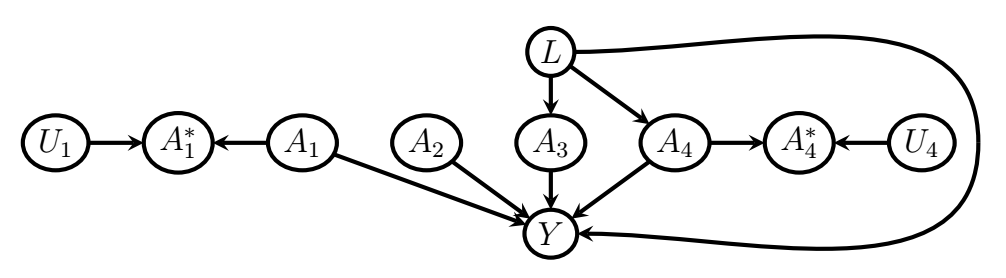
\includegraphics[width=\linewidth]{DAG2_better.png}}
\caption{An example directed acyclic graph (DAG), with variables defined in section 2 and $U$ variables corresponding to measurement error. This DAG represents a scenario with $m=4$ exposures, one each of the following: mismeasured and unconfounded ($A_{1}$), correctly measured and unconfounded ($A_{2}$), correctly measured and confounded ($A_{3}$), and mismeasured and confounded ($A_{4}$). In this case, $A_{2} = A^{*}_{2}$ and $A_{3} = A^{*}_{3}$ since they are both measured without error.}
\label{fig:one}
\end{figure}

The methods proposed in this paper are applicable in settings such as the example directed acyclic graph (DAG) in Figure 1. The methods can accommodate the four types of exposures in the DAG: unconfounded and correctly measured, unconfounded and mismeasured, confounded and correctly measured, and confounded and mismeasured. Here and throughout, exposure measurement error is assumed non-differential with respect to the outcome, e.g., in Figure~\ref{fig:one}, $U_{1}, U_{4} \perp \!\!\! \perp Y$ because the corresponding measured exposures $A^{*}_{1}$ and $A^{*}_{4}$ are colliders on all paths between the errors and the outcome. Many existing methods that adjust for both confounding and measurement biases focus on only mismeasured exposures or on a set of correctly measured exposures with one additional mismeasured exposure; the methods developed in this paper provide a more broadly usable modeling framework where all four types of exposures represented in Figure~\ref{fig:one} can be analyzed simultaneously.

\section{Methods}
\label{s:methods}

The proposed methods combine existing methods for (i) correcting exposure measurement error using CSM and (ii) adjusting for confounding using g-formula, inverse probability weighting, and doubly-robust techniques. To begin, CSM is briefly reviewed.

\subsection{Review of Conditional Score Method}

Suppose the conditional density of the outcome given exposures and covariates is in the exponential family~\citep{mccullagh1989}, i.e., $f(y | \bm{a}, \bm{l}, \Theta) = \exp [ \{y\eta - \mathcal{D}(\eta)\}/ \phi + c(y, \phi) ]$ where $\eta = \beta_{0} + \bm{a}\beta_{a} + \bm{l}\beta_{l}$, $\mathcal{D}$ and $c$ are functions, $\bm{a}$ and $\bm{l}$ are realizations of the random variables $\bm{A}$ and $\bm{L}$, and $\Theta = (\beta_{0}, \beta^{T}_{a}, \beta^{T}_{l}, \phi)$ represents the parameters to be estimated. Assume a classical additive measurement error model $\bm{A}^{*} = \bm{A} + \epsilon_{me}$, where $\epsilon_{me}$ is multivariate normal with mean zero and covariance matrix $\Sigma_{me}$. To account for $A_{j+1}, ...,  A_{m}$ being correctly measured, assume $\Sigma_{me}$ has the block diagonal form
\begin{equation*}
    \Sigma_{me} =
    \begin{bmatrix}
    \Sigma_{e} & 0_{j,m-j} \\
    0_{m-j,j} & 0_{m-j,m-j}
    \end{bmatrix}
\end{equation*}
where $\Sigma_{e}$ is the measurement error covariance matrix for exposures $A_{1},...,A_{j}$ and $0_{a,b}$ denotes an $a \times b$ matrix of zeros.

CSM leverages the fact that $\bm{\Delta} = \bm{A}^{*} + Y(\Sigma_{me}\beta_{a})^{T}/\phi$ is a sufficient statistic for $\bm{A}$. Furthermore, the conditional density of the outcome given covariates and the sufficient statistic is in the exponential family with parameters $\eta_{*} = \beta_{0} + \bm{\delta}\beta_{a} + \bm{l}\beta_{l}$, $\mathcal{D}_{*}(\eta_{*}, \phi, \beta_{a}^{*}) = \phi \log \bigg[ \int \exp \{ y\eta_{*}/\phi + c_{*}(y, \phi, \beta_{a}^{*}) \} dy \bigg]$, and $c_{*}(y, \phi, \beta_{a}^{*}) = c(y, \phi) - \frac{1}{2}(y/\phi)^{2}\beta_{a}^{*}$, where $\bm{\delta}$ is a realization of $\bm{\Delta}$ and $\beta_{a}^{*} = \beta_{a}^{T}\Sigma_{me}\beta_{a}$. This implies that the score equations from the likelihood conditional on $\bm{\Delta}$ yield consistent estimators for $\beta_{a}$ that only depend on the observed data. The form of the score equations depends on the outcome model specification; the general form is
\begin{equation}
    \psi(Y, \bm{L}, \bm{A}^{*}, \Theta) =
    \begin{bmatrix}
       \{ Y - \text{E}(Y | \bm{L}, \bm{\Delta}) \} (1, \bm{L}, \bm{\Delta})^{T} \\
        \phi - \{ Y_{i} - \text{E}(Y | \bm{L}, \bm{\Delta}) \}^{2} / \{ \text{Var}(Y | \bm{L}, \bm{\Delta}) / \phi \}
    \end{bmatrix}
\end{equation}
where $\text{E}(Y | \bm{L}, \bm{\Delta}) = \partial \mathcal{D}_{*} / \partial \eta_{*}$ and $\text{Var}(Y | \bm{L}, \bm{\Delta}) = \phi \partial^{2} \mathcal{D}_{*} / \partial \eta^{2}_{*}$. This procedure can be extended to handle interaction terms~\citep{dagalp2001} by letting $\eta = \beta_{0} + \bm{a}\beta_{a} + \bm{l}\beta_{l} + \bm{a}\beta_{al}\bm{l}^{T}$, where $\beta_{al}$ is an $m \times p$ matrix of interaction parameters, $\bm{\Delta} = \bm{A}^{*} + Y\{ \Sigma_{me}(\beta_{a} + \beta_{al}\bm{L}^{T}) \}^{T}/\phi$, and the appropriate elements of $\beta_{al}$ are constrained to zero such that only relevant interactions are included in the model. Then one can derive estimating equations of the same form as (2), but replacing $(1, \bm{L}, \bm{\Delta})^{T}$ with $(1, \bm{L}, \bm{\Delta}, \bm{L} \otimes \bm{\Delta})^{T}$ where $\bm{L} \otimes \bm{\Delta}$ is a row vector containing the product of the $k^{th}$ element of $\bm{L}$ and the $r^{th}$ element of $\bm{\Delta}$ if and only if the $(r, k)$ element of $\beta_{al}$ is not constrained to be zero.

\subsection{G-formula CSM Estimator}

\sloppy The first proposed method combines the g-formula with CSM. When there is no measurement error, the g-formula estimator is $\hat{E}\{ Y(\bm{a}) \} = n^{-1} \sum_{i=1}^{n} \hat{\text{E}}(Y_{i} | \bm{A} = \bm{a}, \bm{L}_{i})$ where the predicted mean outcomes $\hat{\text{E}}(Y_{i} | \bm{A} = \bm{a}, \bm{L}_{i})$ are typically estimated using parametric models. To accommodate exposure measurement error, the proposed g-formula CSM estimator takes the same form, but instead utilizes a CSM outcome model with relevant covariates and interaction terms. This estimator is a solution to the estimating equation $\sum_{i=1}^{n} \psi_{GF-CSM}(Y_{i}, \bm{L}_{i}, \bm{A}_{i}^{*}, \Sigma_{me}, \Theta_{GF}) = 0$, where
\begin{equation}
    \psi_{GF-CSM}(Y, \bm{L}, \bm{A}^{*}, \Sigma_{me}, \Theta_{GF}) =
    \begin{bmatrix}
       \{ Y - \text{E}(Y | \bm{L}, \bm{\Delta}) \} (1, \bm{L}, \bm{\Delta}, \bm{L} \otimes \bm{\Delta})^{T} \\
        \phi - \{ Y - \text{E}(Y | \bm{L}, \bm{\Delta}) \}^{2} / \{ \text{Var}(Y | \bm{L}, \bm{\Delta}) / \phi \} \\
        g^{-1}(\beta_{0} + \bm{a}\beta_{a} + \bm{L}\beta_{l} +
        \bm{a}\beta_{al}\bm{L}^{T}) - E \{ Y(\bm{a}) \}
    \end{bmatrix}
\end{equation}
and $\Theta_{GF} = (\beta_{0}, \beta^{T}_{a}, \beta^{T}_{l}, vec(\beta_{al}), \phi, E \{ Y(\bm{a}) \})$. To estimate the dose response surface in practice, one can estimate $\hat{E}\{ Y(\bm{a}) \}$ for a large grid of points $\bm{a}$ in the space of interest.

\subsection{IPW CSM Estimator}

Since the CSM estimator can be obtained by solving a set of estimating equations, it's straightforward to define an IPW extension. In particular, consider an estimator of the MSM parameters in (1) that solves $\sum_{i=1}^{n} \psi_{IPW-CSM}(Y_{i}, \bm{L}_{i}, \bm{A}^{*}_{i}, \Sigma_{me}, \Theta_{IPW}) = 0$ where
\begin{equation}
    \psi_{IPW-CSM}(Y, \bm{L}, \bm{A}^{*}, \Sigma_{me}, \Theta_{IPW}) =
    \begin{bmatrix}
       SW \{ Y - E(Y | \bm{\Delta}) \} (1, \bm{\Delta})^{T} \\
       SW \left [ \phi - \{ Y - E(Y | \bm{\Delta})\}^{2} / \{ Var(Y | \bm{\Delta}) / \phi \} \right ]
    \end{bmatrix}
\end{equation}
\begin{equation}
SW = \frac{dF(\bf{A}^{*})}{dF(\bf{A}^{*} | \bm{L})}
\end{equation}
and $\Theta_{IPW} = (\beta_{0}, \beta^{T}_{a}, \beta^{T}_{l}, vec(\beta_{al}), \phi, \gamma)$. The new forms of the conditional expectation and variance follow from setting $\eta_{*} = \gamma_{0} + \bm{\delta}\gamma_{a}$ in the equations in Section 3.1 such that $\hat{\gamma}$ is the solution to (4), along with an additional dispersion parameter estimate. The weights $SW$ are referred to as stabilized weights because of the stabilization properties provided by the density used in the numerator. Since weighting eliminates confounding, the estimating equations of (4) are actually simpler than (2) because covariates $\bm{L}$ do not need to be included in the outcome model.

Methods for fitting MSM with multiple treatments often use weights of the form $SW = \prod_{j=1}^{m} dF(A^{*}_{j}) / dF(A^{*}_{j} | \bm{L})$, e.g., as in \citet{hernan2001}, which assumes that the treatments are independent conditional on $\bm{L}$. This assumption will be made throughout, but it may be dubious in various applications, such as when a treatment has a direct effect on another treatment or when treatments have an unmeasured common cause. For examples of estimating the joint propensity of dependent binary exposures using mixed models, see \citet{tchetgen2012}, \citet{perez2014}, or \citet*{liu2016}. In this setup, if a subset of exposure effects are not subject to confounding, then those exposures do not need to be included in the product defining $SW$.

In practice, the weights $SW$ are usually not known and must be estimated. Models used to estimate weights will be referred to as propensity models and weight components corresponding to continuous exposures will be constructed using a ratio of normal densities estimated from linear models~\citep{hirano2004}. In particular, for a scalar and continuous $A^{*}$, a model of the form $A = \alpha (1, \bf{L})^{T} + \epsilon_{ps}$ where $\epsilon_{ps} \sim \mathcal{N}(0, \sigma^{2}_{ps})$ would be fit, and $\hat{\alpha}$ and $\hat{\sigma}_{ps}$ would yield a conditional density $\hat{f}(A^{*}|\bf{L})$. This density evaluated at each individual's exposure value gives the weight denominators. An intercept-only model is used similarly to calculate the weight numerators. Other methods and more flexible choices for weight models~\citep{naimi2014} can also be used for continuous exposures in practice. An additional challenge arises when estimating weights in that the exposure measurement error has another opportunity to introduce bias. Fortunately, the exposures are now the propensity model(s) outcomes, and measurement error is usually much less serious for a model outcome than for model covariates~\citep{carroll2006}. In Web Appendix A, the proposed IPW CSM estimator is shown to be consistent even when the propensity models are fit using the mismeasured exposures without correction, under certain assumptions.

\subsection{Doubly-Robust CSM Estimator}

Both g-formula and IPW methods rely on model specifications that may not be correct in practice. The g-formula provides consistent estimation of potential outcome means only when the outcome model with exposures and confounders is correctly specified. Likewise, IPW estimators are consistent only when the propensity score models are correctly specified. In contrast, doubly-robust (DR) estimators entail specifying both propensity and outcome models, but remain consistent if one is misspecified and the other is not (\citealp*{robins1994}; \citealp{lunceford2004,bang2005}).

A DR estimator for the additive measurement error setting can be derived as an extension of the procedure referred to as doubly-robust standardization in \citet{vansteelandt2011}, which was covered in detail for binary treatments in \citet{hirano2001} and \citet{kang2007}. Namely, one can perform the g-formula using a weighted outcome regression where the weights are the inverse probability weights given in equation (5). This DR estimator is a solution to the estimating equation $\sum_{i=1}^{n} \psi_{DR-CSM}(Y_{i}, \bm{L}_{i}, \bm{A}_{i}^{*}, \Sigma_{me}, \Theta_{DR}) = 0$, where $\Theta_{DR} = \Theta_{GF}$ and
\begin{equation}
    \psi_{DR-CSM}(Y, \bm{L}, \bm{A}^{*}, \Sigma_{me}, \Theta_{DR}) =
    \begin{bmatrix}
       SW\{ Y - \text{E}(Y | \bm{L}, \bm{\Delta}) \} (1, \bm{L}, \bm{\Delta}, \bm{L} \otimes \bm{\Delta})^{T} \\
        SW[\phi - \{ Y - \text{E}(Y | \bm{L}, \bm{\Delta}) \}^{2} / \{ \text{Var}(Y | \bm{L}, \bm{\Delta}) / \phi \}] \\
        g^{-1}(\beta_{0} + \bm{a}^{*}\beta_{a} + \bm{L}\beta_{l} +
        \bm{a}^{*}\beta_{al}\bm{L}^{T}) - E \{ Y(\bm{a}) \}
    \end{bmatrix}
\end{equation}
This estimator will be referred to as the DR CSM estimator. If the stabilized weights $SW$ are unknown, they can be estimated as described for the IPW CSM estimator. Like the g-formula CSM estimator, the DR CSM estimator can be evaluated over a grid of values $\bm{a}$ of interest to estimate a dose-response surface.

A second DR estimator, similar to those described in \citet{robins2000b} and \citet{neugebauer2005}, is given by the solution to the set of estimating equations $\sum_{i=1}^{n} \psi_{DR-CSM-alt}(Y_{i}, \bm{L}_{i}, \bm{A}^{*}_{i}, \Theta_{DR-alt}) = 0$ where $\Theta_{DR-alt} = \Theta_{IPW}$ and
\begin{equation*}
    \psi_{DR-CSM-alt}(Y, \bm{L}, \bm{A}^{*}, \Theta_{DR-alt}) =
    \begin{bmatrix}
       SW \{ Y - E(Y | \bm{\Delta}) - Q(\bm{A}^{*}, \bm{L}) \} + \int_{\bm{a}} h(\bm{a})Q(\bm{a}, \bm{L})d\mu (\bm{a}) \\
       SW \{ Y - E(Y | \bm{\Delta}) - Q(\bm{A}^{*}, \bm{L}) \} \bm{\Delta} + \int_{\bm{a}} h(\bm{a})Q(\bm{a}, \bm{L})d\mu (\bm{a})
    \end{bmatrix},
\end{equation*}
$h(\bm{a})$ is the numerator of the stabilized weights, $d\mu (\bm{a})$ is a Lebesgue measure, and $Q(\bm{A}, \bm{L}) = \beta_{0} + \bm{A} \beta_{a} + \bm{L} \beta_{l} + \bm{A} \beta_{al}\bm{L}^{T} - \gamma (1, \bm{A})^{T}$ when the outcome regression is correctly specified. Note the second DR estimator targets the same MSM parameter estimand as the IPW estimator. Thus the outcome regression model must be compatible with the assumed MSM of the dose-response surface; otherwise mis-specification is guaranteed. The second DR estimator makes key three assumptions: a propensity model, an outcome model, and a MSM. It is consistent if either (i) the MSM and propensity model are correctly specified or (ii) the MSM and outcome model are correctly specified. On the other hand, the DR CSM estimator does not assume a MSM form and is consistent if either the propensity model or outcome model is correctly specified. For this reason, the DR CSM estimator may be preferred in this setting.

\subsection{Handling Unknown Measurement Error Variance}

Although the proposed methods require no supplemental data and no distributional assumption on the true exposures $\bm{A}$, a priori knowledge of the measurement error covariance matrix is required. Sometimes this matrix will be known from properties of the measurement devices (e.g., some bioassays, certain widely studied survey instruments) or will be available from a prior study. Here, some guidelines are provided for analyses where this matrix is unknown.

Firstly, there are many types of studies for which the covariance matrix should be diagonal (i.e., the measurement errors should be uncorrelated). For example, biological assays run on different samples and analyzed by separate machines/researchers should have uncorrelated measurement errors, and different assays run on the same sample may often have uncorrelated or very weakly correlated measurement errors. For other types of data such as survey responses, analysts should be more cautious, noting that response bias, recall bias, and other forms of measurement error in survey instruments may be correlated within individuals.

Some studies may have available supplemental data in the form of replicates of the potentially mismeasured variables. These replicates can be used to estimate $\Sigma_{me}$ as described in \citet{carroll2006}. Suppose there are $k_{i}$ replicates of the mismeasured exposures, $\bm{A}^{*}_{i1}, ..., \bm{A}^{*}_{ik_{i}}$ with mean for individual $i$ notated as $\bm{A}^{*}_{i.}$. Then an estimator for the measurement error covariance is given by:
\begin{equation*}
    \hat{\Sigma}_{me} = \frac{\sum_{i=1}^{n} \sum_{j=1}^{k_{i}} (\bm{A}^{*}_{ij} - \bm{A}^{*}_{i.})^{T}(\bm{A}^{*}_{ij} - \bm{A}^{*}_{i.})}{\sum_{i=1}^{n}(k_{i} - 1)}
\end{equation*}
When replicates are available, some of the existing methods described in the introduction are applicable and should give similar results to the proposed methods.

When no replicates are available and there is no prior knowledge of $\Sigma_{me}$, the proposed methods can still be used in conjunction with a sensitivity analysis. In some settings, an upper bound on the exposure measurement error variance may be assumed; for example, the variance of a correctly measured exposure (if estimated in a prior study) can act as a reasonable upper bound on measurement error variance for the corresponding mismeasured exposure. Once upper bounds are determined, inference may be repeated using the proposed methods for a range of $\Sigma_{me}$ specifications to assess robustness of point estimates and confidence intervals to the degree of assumed measurement error; this procedure is more straightforward when the matrix is small and diagonal, and becomes difficult to interpret as the number of non-zero parameters grows.

\subsection{Large-Sample Properties and Variance Estimation}

In Web Appendix A, each of the three proposed estimators are shown to be consistent and asymptotically normal by showing that their corresponding estimating functions have expectation 0~\citep{stefanski2002}. In addition, the DR CSM estimator is shown to be consistent when only one of the propensity and outcome models is correctly specified. Finally, the proposed estimators are shown to be generalizations of existing popular estimators used in the no measurement error setting.

Since each proposed estimator is an M-estimator, consistent estimators of their asymptotic variances are given by the empirical sandwich variance technique. Estimating equations corresponding to the estimation of weights (and $\hat{\Sigma}_{me}$ if estimated) should be included in the estimating equation vector for each method when computing the sandwich variance estimator. Wald $100(1-\alpha)\%$ confidence intervals for the parameters of interest can then be constructed in the usual fashion. The geex R package~\citep{saul2017} streamlines variance estimation for M-estimators and is used in the simulation and application sections.

\section{Simulation Study}

The performance of the proposed methods was evaluated in three simulation studies. The first simulation compared the proposed g-formula CSM approach to standard methods in a scenario where confounding and additive exposure measurement error were present. A total of 2000 data sets of $n = 800$ individuals were simulated, each with the following variables: a confounder $L_{1}$ simulated as a Bernoulli random variable with expectation $0.5$, i.e., $L_{1} \sim \text{Bern}(0.5)$; a second confounder $L_{2} \sim \text{Bern}(0.2)$; an exposure $A \sim \mathcal{N}(2 + 0.3L_{1} - 0.5L_{2}, 0.6)$; and an outcome $Y \sim \text{Bern}(\text{logit}^{-1}(-2 + 0.7A - 0.6L_{1} + 0.4L_{2} - 0.4AL_{1} - 0.2AL_{2}))$. The exposure was subject to additive measurement error, simulated as $A^{*} \sim \mathcal{N}(A, \sigma^{2} = 0.25)$.

Dose-response curves were estimated using four methods: (i) logistic regression specifying Y as a function of $A^{*}, L_{1}, L_{2}$ and the interactions between $A^{*}$ and each covariate; (ii) CSM with the same outcome specification as the logistic regression and correctly specified measurement error variance; (iii) the g-formula with a correctly specified outcome model using the mismeasured exposures; and (iv) the proposed g-formula CSM estimator with a correctly specified outcome regression. For the point on the true dose response curve $E\{ Y(a = 3) \}$, the average bias, average estimated standard error, empirical standard error, and percentage of estimated confidence intervals covering the true value were estimated across the 2000 simulation runs.

Biases of the estimated dose-response curves are displayed in Figure~\ref{fig:two}. Only the proposed g-formula CSM estimator was approximately unbiased. In contrast, the other three methods performed poorly with high bias across nearly the entire range of exposure values evaluated. This is expected because these methods do not adjust for both confounding and measurement error. Likewise, only the proposed g-formula CSM estimator was unbiased with corresponding confidence intervals achieving nominal coverage for the potential outcome mean at $a = 3$ on the dose-response curve, as summarized in Table~\ref{tab:one}.

\begin{figure}
\centering
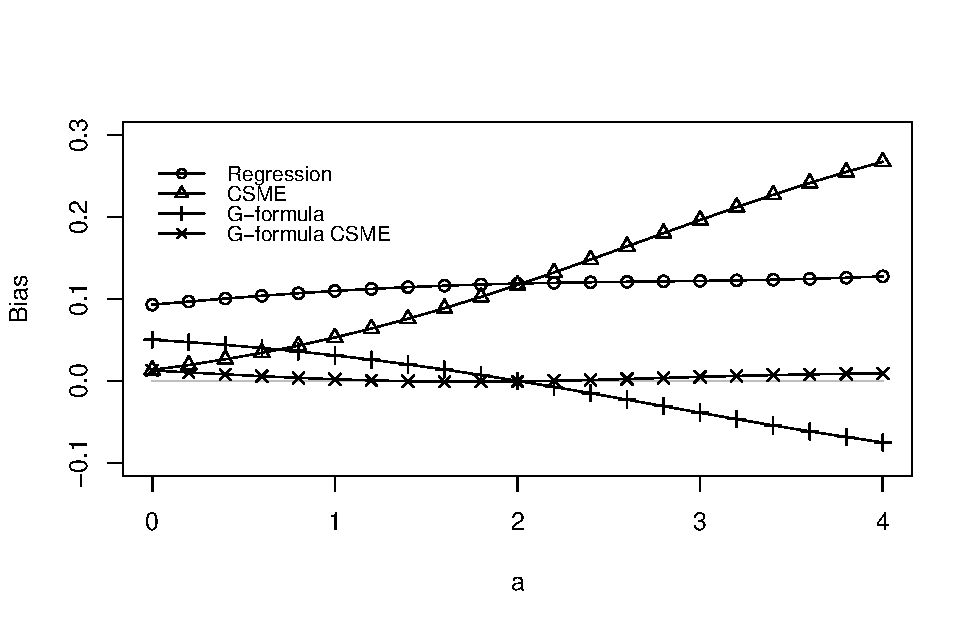
\includegraphics[width=6in]{paper1-fig2-grey.pdf}
\caption{Estimated dose-response curve bias for each of the four methods compared in the first simulation study. Bias refers to the average bias across 2,000 simulated data sets for each method evaluated at each point on the horizontal axis $a = (0, 0.2, 0.4, ..., 4)$. The gray horizontal line corresponds to zero bias.}
\label{fig:two}
\end{figure}

The second simulation study compared the proposed IPW CSM approach to standard methods. A total of 2000 data sets of $n = 800$ individuals were simulated, each with the following variables: a confounder $L \sim \text{Exp}(\lambda = 3)$, first true exposure $A_{1} \sim \mathcal{N}(4 + 0.9L, 1.1)$, second true exposure $A_{2} \sim \mathcal{N}(2.5, 0.7)$, third true exposure $A_{3} \sim \mathcal{N}(1.4 + 0.5, 0.6)$ and an outcome $Y \sim \text{Bern}(\exp(-1.7 + 0.4A_{1} - 0.4A_{2} - 0.6A_{3} + 0.7L - 0.6A_{1}L - 0.9A_{3}L - \log(\lambda / (\lambda - 0.7 + 0.6A_{1} + 0.9A_{3}))) / (1 + \exp(-1.7 + 0.4A_{1} - 0.4A_{2} - 0.6A_{3})))$ such that $\text{logit}[E\{ Y(a_{1}, a_{2}, a_{3})\} ] = \gamma_{0} + \gamma_{1}a_{1} + \gamma_{2}a_{2} + \gamma_{3}a_{3} = -1.7 + 0.4a_{1} - 0.4a_{2} - 0.6a_{3}$. The third exposure $A_{3}$ was allowed to be correctly measured, while $A_{1}$ and $A_{2}$ were subject to additive measurement error simulated as $A_{1}^{*} \sim \mathcal{N}(A_{1}, 0.36)$ and $A_{2}^{*} \sim \mathcal{N}(A_{2}, 0.25)$ (i.e., the measurement error covariance matrix was diagonal).

\begin{table}[]
    \centering
    %\footnotesize
    \caption{Results from the first simulation study. Bias: 100 times the average bias across simulated data sets for each method; ASE: 100 times the average of estimated standard errors; ESE: 100 times the standard deviation of parameter estimates; Cov: Empirical coverage of 95$\%$ confidence intervals for each method, rounded to the nearest integer.}
    \begin{tabular}{lrrrr}
    \hline
         Estimator & Bias & ASE & ESE & Cov \\
         \hline
         %\hhline{|=|=|=|=|=|=|}
Regression & -51.5 & 18.3 & 18.3 & 19\% \\
CSM & -21.8 & 28.4 & 28.6 & 87\% \\
G-formula & -3.9 & 2.6 & 2.6 & 67\% \\
G-formula CSM & 0.5 & 4.0 & 4.1 & 95\% \\
         \hline
    \end{tabular}
    \label{tab:one}
\end{table}

The MSM parameters of interest $\gamma_{1}$, $\gamma_{2}$, and $\gamma_{3}$ were estimated from the observed data $\{ Y, A_{1}^{*}, A_{2}^{*}, A_{3}, L \}$ using four methods: (i) logistic regression specifying Y as a function of $A_{1}^{*}, A_{2}^{*}, A_{3}, L$ and the interactions between $A_{1}^{*}$ and $L$ as well as $A_{3}$ and $L$; (ii) the CSM method with the same outcome specification as the logistic regression and correctly specified measurement error variances; (iii) an IPW estimator where a correctly specified propensity model was fit for both $A_{1}^{*}$ and $A_{3}$ and the product of the resulting inverse probability weights were used to weight a logistic regression of $Y$ on the three observed exposures; and (iv) the proposed IPW CSM estimator using correctly specified measurement error variances and weights from correctly specified propensity models.

\begin{table}[]
    \caption{Results from the second simulation study. Bias, ASE, ESE, and Cov defined as in Table 1.}
    \begin{center}
    \begin{tabular}{clrrrr}
    \hline
        Parameter & Estimator & Bias & ASE & ESE & Cov \\
         \hline
$\gamma_{1}$ & Regression & 5.8 & 13.6 & 13.3 & 93\% \\
$\gamma_{1}$ & CSM & 22.0 & 19.2 & 18.7 & 80\% \\
$\gamma_{1}$ & IPW & -9.7 & 9.1 & 9.0 & 80\% \\
$\gamma_{1}$ & IPW CSM & 0.3 & 12.5 & 12.3 & 95\% \\[4pt]
$\gamma_{2}$ & Regression & 11.7 & 13.3 & 13.0 & 84\% \\
$\gamma_{2}$ & CSM & -3.9 & 21.1 & 20.5 & 95\% \\
$\gamma_{2}$ & IPW & 13.8 & 13.3 & 12.9 & 80\% \\
$\gamma_{2}$ & IPW CSM & -0.3 & 20.7 & 20.1 & 95\% \\[4pt]
$\gamma_{3}$ & Regression & 10.4 & 27.9 & 27.4 & 92\% \\
$\gamma_{3}$ & CSM & 9.2 & 28.9 & 27.8 & 92\% \\
$\gamma_{3}$ & IPW & 0.3 & 19.8 & 19.4 & 94\% \\
$\gamma_{3}$ & IPW CSM & -0.4 & 20.1 & 19.7 & 95\% \\
         \hline
    \end{tabular}
    \end{center}
    \label{tab:two}
\end{table}

The average bias, average estimated standard error, empirical standard error, and percentage of confidence intervals covering the true values across the 2000 simulation runs are presented in Table~\ref{tab:two}. For $\gamma_{2}$, the parameter corresponding to the mismeasured but unconfounded exposure, methods (ii) and (iv) achieved near-zero average bias and approximately nominal coverage, while methods (i) and (iii) were biased and had lower coverage. For $\gamma_{3}$, the parameter corresponding to the confounded but correctly measured exposure, methods (iii) and (iv) achieved low bias and about nominal coverage, while methods (i) and (ii) performed poorly. For $\gamma_{1}$, the parameter corresponding to the mismeasured and confounded exposure, only the method proposed in this paper (iv) had approximately 0 bias and nominal coverage.

The third simulation study compared the proposed g-formula and IPW CSM approaches to the proposed DR CSM estimator under various model specifications. In particular, 2000 datasets of $n = 2000$ individuals were simulated with the following variables: a confounder $L_{1} \sim \text{Binom}(0.5)$, a second confounder $L_{2} \sim \mathcal{N}(1, 0.5)$, an exposure $A \sim \mathcal{N}(2 + 0.9L_{1} - 0.6L_{2}, 1.1)$, and a continuous outcome $Y \sim \mathcal{N}(1.5 + 0.7A + 0.9L_{1} - 0.7AL_{1} - 0.6L_{2} + 0.4AL_{2})$ such that the assumptions of all three methods held. The methods were compared in performance estimating the coefficient for $a$ in the marginal structural model resulting from these distributional assumptions. The exposure $A$ was subject to additive measurement error simulated as $A^{*} \sim \mathcal{N}(A, 0.16)$. Then the three approaches were compared under scenarios where only the propensity model was correctly specified, only the outcome regression was correctly specified, and where both were correctly specified. The propensity model was mis-specified by not including the confounder $L_{1}$ and the outcome regression was mis-specified by leaving out $L_{1}$ and the interaction between $A$ and $L_{1}$.

\begin{table}[]
    \centering
    %\footnotesize
    \caption{Results from the third simulation study. Bias, ASE, ESE, and Cov defined as in Table 1. PS indicates the propensity score model is correctly specified; OR indicates the outcome regression is correctly specified.}
    \begin{tabular}{lcrrrr}
    \hline
         Estimator & Correct Specifications & Bias & ASE & ESE & Cov \\
         \hline
         %\hhline{|=|=|=|=|=|=|}
G-formula CSM & PS & -6.6 & 1.9 & 1.9 & 8\% \\
IPW CSM & PS & 0.0 & 3.2 & 3.1 & 95\% \\
DR CSM & PS & 0.0 & 2.6 & 2.6 & 94\% \\[4pt]
G-formula CSM & OR & 0.0 & 1.7 & 1.7 & 94\% \\
IPW CSM & OR & -6.3 & 2.0 & 2.0 & 12\% \\
DR CSM & OR & 0.1 & 1.7 & 1.7 & 95\% \\[4pt]
G-formula CSM & PS and OR & 0.0 & 1.7 & 1.7 & 94\% \\
IPW CSM & PS and OR & 0.0 & 3.2 & 3.1 & 95\% \\
DR CSM & PS and OR & 0.1 & 1.9 & 1.9 & 94\% \\
         \hline
    \end{tabular}
    \label{tab:three}
\end{table}

The simulation results are presented in Table~\ref{tab:three} and match the theoretical results described in Section 3.4. Namely, when only the propensity score model was specified correctly, the IPW estimator performed well, but the g-formula estimator was subject to substantial bias and undercoverage. Likewise when only the outcome model was specified correctly, the g-formula estimator performed well, but the IPW estimator was biased and had lower than nominal coverage. However, the doubly-robust estimator achieved low bias and approximately nominal coverage when only one of the two models was misspecified, exhibiting its namesake double-robustness property.

\section{Application}

To illustrate the proposed methods, the DR CSM estimator was applied to data from the HVTN 505 vaccine trial. As discussed in the Introduction, the candidate HIV vaccine studied in this trial was not effective, but follow-up research described several interesting biomarker correlates of risk. Recently \citet{neidich2019} investigated potential mechanisms of antibody mediated prevention, finding that antibody-dependent cellular phagocytosis and antigen-specific recruitment of Fc$\gamma$ receptors of several HIV-1 specific Env proteins were associated with reduced HIV-1 risk.

In this section, the primary analysis of \citet{neidich2019} is reassessed by (i) adjusting for measured potential confounders beyond simple inclusion in an outcome regression, (ii) allowing for additive measurement error, and (iii) estimating full dose-response curves rather than coefficients from logit-linear models. Attention is focused on the log transforms of markers measuring antibody-dependent cellular phagocytosis and recruitment of Fc$\gamma$R\RNum{2}a of the H131-Con S gp140 protein, which will be referred to as ADCP and R\RNum{2}. The primary analysis of \citet{neidich2019} focused on the effect of each of these exposures individually on HIV-1 acquisition among vaccinees. For each exposure, they fit a logistic regression model and reported odds ratios for the main effect of exposure adjusting for age, BMI, race, and behavior risk, as well as CD4 and CD8 polyfunctionality scores (CD4-P and CD8-P).

In this section, the data is analyzed making the same Binomial family distribution assumption for the outcome and using the proposed doubly-robust CSM estimator. To account for the two-phase sampling design used in the HVTN 505 trial, the weights in the doubly-robust estimator are multiplied by inverse probability of sampling weights, following the procedure described in \citet{wang2009}. This version of the proposed estimator is described in more detail and evaluated in a simulation study in Web Appendix B. ADCP and R\RNum{2} were modeled separately to match the univariate-style analysis performed in \citet{neidich2019}. For the propensity model specification, main effects for baseline covariates age, race, BMI, behavior risk, CD4-P, and CD8-P were included. For the outcome model specification, main effects for the exposure of interest, age, race, BMI, behavior risk, CD4-P, and CD8-P were included, along with interactions of the exposure with age and the exposure with behavior risk. Based on the theoretical and empirical results in sections 3 and 4, the estimator should be consistent if either specification is correct. Finally, each exposure was assumed to follow a classical additive measurement error model where a sensitivity analysis was performed by varying the measurement error variances from 0 to 1/6, 1/4, and 1/3 of the variance for each exposure variable when restricted to vaccinees with an immune response. Since ADCP and R\RNum{2} are log-transformations of strictly positive random variables, this setup is equivalent to assuming that their corresponding non-log transformed variables follow multiplicative measurement error models. Dose response curves were estimated for each exposure and each measurement error level across ranges of exposure values containing almost all data points, but excluding outliers.

\begin{figure}[h!]
\centering
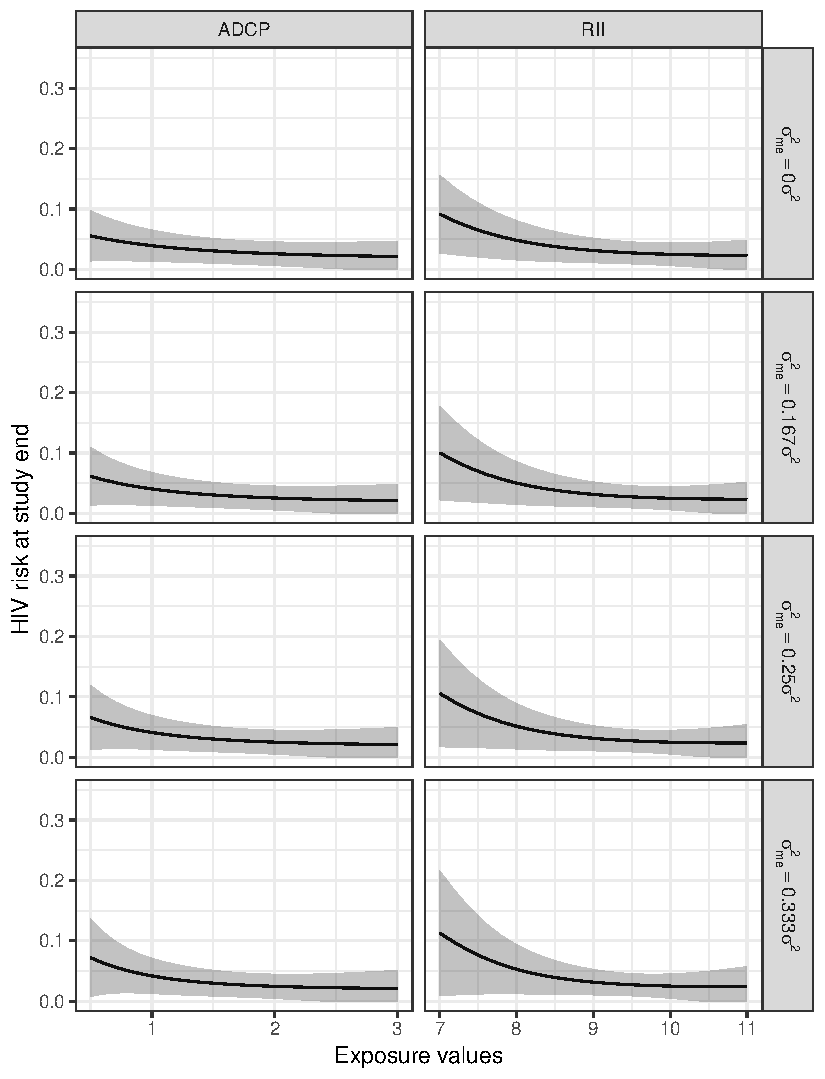
\includegraphics[width=5.6in]{fig3-updated.pdf}
\caption{HVTN 505 results. Each panel shows the dose-response curve for ADCP or R\RNum{2} estimated by the DR CSM estimator, as well as their respective shaded confidence regions. From top to bottom, each panel reflects increasing user-specified variances of measurement error $\sigma^{2}_{me}$ corresponding to proportions of 0, 1/6, 1/4, and 1/3 of $\sigma^{2}$, the estimated total exposure variances among vaccinees with immune responses. Lower confidence limits that were estimated to be negative were truncated at 0.}
\label{fig:three}
\end{figure}

The analysis results are plotted in Figure~\ref{fig:three}. For each exposure, lower values corresponded to higher HIV risk among the trial population, in line with prior results and biological theory. Moving across panels from top to bottom, the assumed measurement error variance increases and the confidence regions become wider, as expected. While there appears to be evidence that higher levels of each exposure are protective, there is a lot of uncertainty when allowing for higher magnitudes of measurement error and because of the low sample size in general. This provides further evidence that future vaccine candidates designed to elicit strong ADCP and R\RNum{2} responses may confer some protection, but that studies with more participants with biomarkers measured are needed to draw stronger conclusions.

\section{Discussion}

In this paper, estimators are proposed which adjust for both confounding and measurement error and which are consistent without any supplemental data and without specifying strong distributional or extrapolation assumptions. The proposed methods are semi-parametric in that while parametric assumptions for the errors were made, no assumptions were made about the distributions of true exposures. Another notable contribution of this paper is to provide an R package with code examples for the conditional score method, which have not previously been provided in even the standard (not causal inference focused) setting.

While the proposed methods were shown to have favorable theoretical and empirical properties, they are not without limitation. In particular, the methods only work without supplemental data if the covariance of measurement error is known or has been previously estimated. As demonstrated in Section 5, if the covariance is unknown then sensitivity analysis can be straightforward and highly informative if the covariance matrix is small or restricted such that it has few parameters. In addition, in order to perform inference without making strong assumptions on $\bm{A}$, modeling assumptions on $\bm{A}^{*}$ and $Y$ that may be implausible in some settings were necessary. However, additive measurement error models are realistic for many variables and the generalized linear model framework assumed for the outcome is an extremely common statistical analysis procedure used in many fields. Simulations of the proposed methods under violations of the positivity and additive measurement error assumptions are presented in Web Table 2 and Web Table 3.

There are several possible extensions of the methods described in this paper. Methods that accommodate different measurement error model forms and more flexible outcome model specifications would be useful. Generalizations of the conditional score approach to broader semiparametric frameworks such as that described in \citet{tsiatis2004} could be adapted to the causal setting to address this and weaken some of the parametric assumptions made in this paper. A version of this idea is proposed by \citet{liu2017}, but the authors take an outcome regression approach to adjusting for confounding, which is often insufficient for causal inference.

Another logical extension would be a g-estimation based estimator that builds off CSM to estimate parameters of a structural nested model where at least one exposure is measured with error. In addition, while this paper expands on the conditional score estimation procedure described in \citet{stefanski1987}, the corrected score estimation procedure described in \citet{nakamura1990} also belongs to the score equation family of functional methods, can also correct for measurement error without supplemental data, and has advantages and disadvantages compared to the conditional score approach in various settings. A causal extension of the corrected-score approach would be valuable for many applications. Finally, this paper focuses on point-exposure data, but conditional-score based approaches addressing measurement error and data sparsity for longitudinal and survival data have been described and could be extended to define new causal inference methods in those settings.

This paper adds to a growing literature on addressing measurement error in causal inference problems. No measurement error of any variables is a key assumption in drawing causal inference, but is often left implicit in analyses despite being critical to the identification of causal estimands. Indeed, exposure measurement error is common in observational studies where investigators lack control of the exposure variables - the same conditions in which investigators worry about confounding bias. Methodological contributions at this intersection are needed to facilitate simultaneous adjustment for these prevalent issues.

%  The \backmatter command formats the subsequent headings so that they
%  are in the journal style.  Please keep this command in your document
%  in this position, right after the final section of the main part of
%  the paper and right before the Acknowledgements, Supplementary Materials,
%  and References sections.




\backmatter

%  This section is optional.  Here is where you will want to cite
%  grants, people who helped with the paper, etc.  But keep it short!

\section*{Acknowledgements}

The authors thank Kayla Kilpatrick, Shaina Mitchell, Sam Rosin, Bonnie Shook-Sa, and Jaffer Zaidi for helpful comments and suggestions, as well as the investigators, staff, and participants of the HVTN 505 trial. This work was supported by NIH grant R37 AI054165. \vspace*{-8pt}

%  Here, we create the bibliographic entries manually, following the
%  journal style.  If you use this method or use natbib, PLEASE PAY
%  CAREFUL ATTENTION TO THE BIBLIOGRAPHIC STYLE IN A RECENT ISSUE OF
%  THE JOURNAL AND FOLLOW IT!  Failure to follow stylistic conventions
%  just lengthens the time spend copyediting your paper and hence its
%  position in the publication queue should it be accepted.

%  We greatly prefer that you incorporate the references for your
%  article into the body of the article as we have done here
%  (you can use natbib or not as you choose) than use BiBTeX,
%  so that your article is self-contained in one file.
%  If you do use BiBTeX, please use the .bst file that comes with
%  the distribution.

\bibliographystyle{biom}
\bibliography{refs}

%\begin{thebibliography}{}

%\end{thebibliography}

%  If your paper refers to supplementary web material, then you MUST
%  include this section!!  See Instructions for Authors at the journal
%  website http://www.biometrics.tibs.org

\section*{Supporting Information}

Web Appendices, Tables, and Figures referenced in Sections 3 and 6 are available with this paper at the Biometrics website on Wiley Online Library. All R code used in the simulations and application is available at \href{https://github.com/bblette1/causalCSME}{https://github.com/bblette1/causalCSME}. (Will edit this after talking to Peter) The data that support the findings of this study are openly available in [repository name] at [URL], reference number [reference number].\vspace*{-8pt}

\label{lastpage}

\end{document}

